\section{KNN}
KNN is a supervised. The method is non parametric meaning that the method does not make any assumption about the distribution of the data. The method is also labeled as lazy learning, as the it does not use any training points to do any generalization.\\

\begin{figure}[H]
\centering
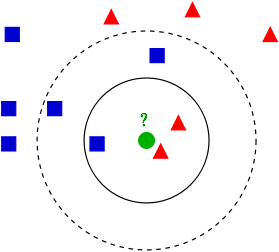
\includegraphics[width = 0.3\textwidth]{img/kNN-classification.png}
\caption{kNN classification  - the green circles has to be classified between the two classes indicated as red triangles and blue squares. k= 3}
\end{figure}

The purpose of this algorithm is to classify a new object based on its attributes and the training samples that has been used. The algorithm decides which class a new object belongs to by inspecting the k nearest neighbours, and based on the class which is the majority, will the class of the new object be determined. The number of k can be either a even or odd number, in the case of a tie with a even numbered k will the class be randomly be decided amongst the two competing ones, one have to choose the optimal value for k  in order to get an accurate predictor. The distance between two can be computed different ways, such as \\

\textbf{Euclidian distance}

\begin{equation}
d(\overrightarrow{w},\overrightarrow{v}) = \sqrt{\sum_{i}^n (w_i - v_i)^2}
\end{equation}

\textbf{Manhattan distance}

\begin{equation}
d(\overrightarrow{w},\overrightarrow{v}) = \sum_{i}^n (w_i - v_i)
\end{equation}

The advantages of using kNN is that it is simple to use, and works well on basic problems however it can be slow in for real-time prediction especially if the dataset used for training is large, as the method is a lazy learner.Another disadvantage of the method is that it does not learn anythign from the trainings data, but just stores them.  The method is not in particular robust against noisy data.    